\let\negmedspace\undefined
\let\negthickspace\undefined
\documentclass[journal]{IEEEtran}
\usepackage[a5paper, margin=10mm, onecolumn]{geometry}
%\usepackage{lmodern} % Ensure lmodern is loaded for pdflatex
\usepackage{tfrupee} % Include tfrupee package

\setlength{\headheight}{1cm} % Set the height of the header box
\setlength{\headsep}{0mm}     % Set the distance between the header box and the top of the text

\usepackage{gvv-book}
\usepackage{gvv}
\usepackage{cite}
\usepackage{amsmath,amssymb,amsfonts,amsthm}
\usepackage{algorithmic}
\usepackage{graphicx}
\usepackage{textcomp}
\usepackage{xcolor}
\usepackage{txfonts}
\usepackage{listings}
\usepackage{enumitem}
\usepackage{mathtools}
\usepackage{gensymb}
\usepackage{comment}
\usepackage[breaklinks=true]{hyperref}
\usepackage{tkz-euclide} 
\usepackage{listings}
% \usepackage{gvv}                                        
\def\inputGnumericTable{}                                 
\usepackage[latin1]{inputenc}                                
\usepackage{color}                                            
\usepackage{array}                                            
\usepackage{longtable}                                       
\usepackage{calc}                                             
\usepackage{multirow}                                         
\usepackage{hhline}                                           
\usepackage{ifthen}                                           
\usepackage{lscape}
\begin{document}

\bibliographystyle{IEEEtran}
\vspace{3cm}

\title{4-4.2-3}
\author{AI24BTECH11003 - Vijaya Sreyas
}
% \maketitle
% \newpage
% \bigskip
{\let\newpage\relax\maketitle}

\renewcommand{\thefigure}{\theenumi}
\renewcommand{\thetable}{\theenumi}
\setlength{\intextsep}{10pt} % Space between text and floats


\numberwithin{equation}{enumi}
\numberwithin{figure}{enumi}
\renewcommand{\thetable}{\theenumi}


\textbf{Question}:\\
Find the direction and normal vectors of the following line: $-2x+3y=6$

\textbf{Solution: }

\begin{table}[h!]    
  \centering
  \begin{tabular}[12pt]{|c|c|l|}
    \hline
	\textbf{Point} & \textbf{Position} & \textbf{Description}\\ 
    \hline
	\textbf{A} & $\myvec{x \\ y}$ & Unknown end of a diameter \\
    \hline 
	\textbf{B} & $\myvec{1 \\ 4}$ & Known end of diameter \\
    \hline
	\textbf{O} & $\myvec{2 \\ -3}$ & Center of the circle \\
    \hline   
    \end{tabular}

  \caption{Final Information}
  \label{4-4.2-3-tab-0}
\end{table}

The equation of the given line is:
\begin{align}
    6 &= -2x + 3y \\
    y &= 2 + \frac{2}{3}x \\
    \implies \myvec{x \\ y} &= \myvec{x \\ \frac{2}{3}x + 2} = \myvec{0 \\ 2} + x\myvec{1 \\ \frac{2}{3}} \\
	\vec{X} &= \vec{h} + k\vec{m}
\end{align}

Thereby yielding the direction vector:
\begin{align}
    \vec{m} &= \myvec{1 \\ \frac{2}{3}} 
\end{align}

From \eqref{eq:line-school-dir} and \eqref{line-school-normal}, we get:
\begin{align}
    \vec{n} &= \myvec{-\frac{2}{3} \\ 1}
\end{align}

Therefore, the direction vector of the line can be given by $\vec{m} = \myvec{3 \\ 2}$ and the normal vector by $\vec{n} = \myvec{-2 \\ 3}$.

\begin{figure}[H]
    \centering
    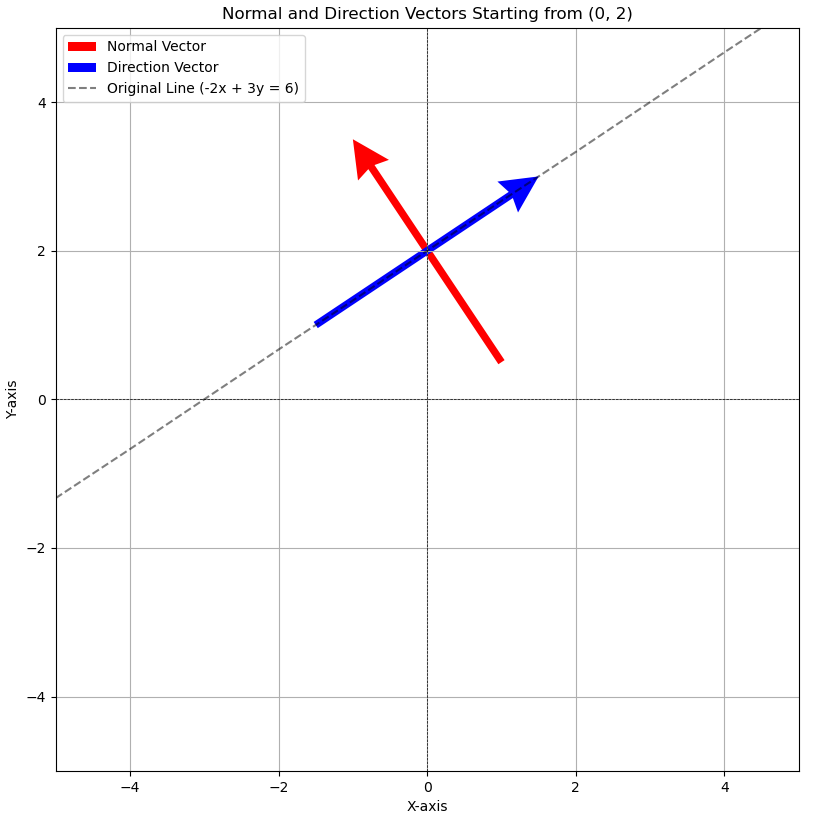
\includegraphics[width=0.7\columnwidth]{figs/Figure_1.png}
    \caption{Line and Vectors}
    \label{4-4.2-3-fig-0}
\end{figure}

\end{document}


